\subsection{One Multinomial Sampling with $n$ Fixed}
The contingency Table for this design is as follows
\begin{figure}[H]
	\centering
	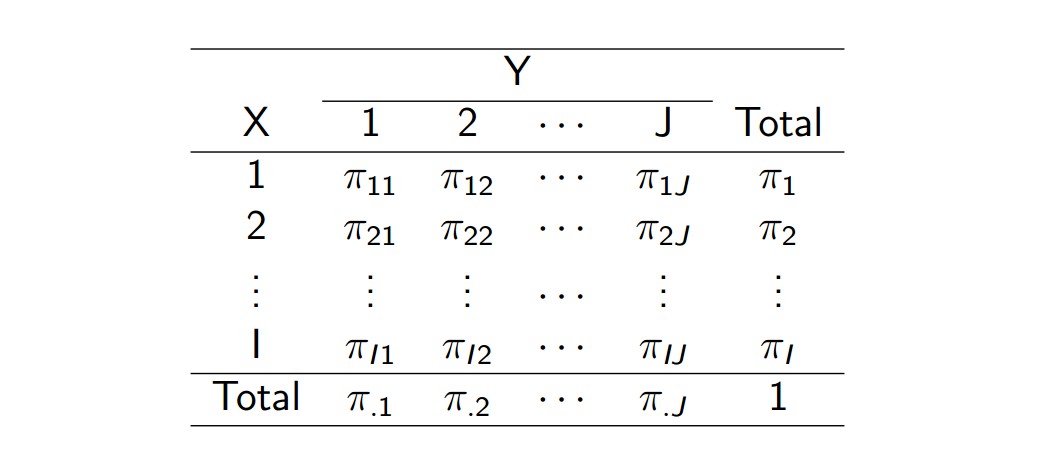
\includegraphics[width=0.7\linewidth]{fig/screenshot002}
	\caption{Example of Contingency Table}
	\label{fig:screenshot002}
\end{figure}

Here $\pi_{ij} = \P(X = i, Y = j)$ is the probability that $(X, Y)$ falls in the $ij$-th cell. The combinations of $\pi_{ij}$'s form the joint distribution of $X$ and $Y$.
\[\sum_{i=1}^{I} \sum_{j=1}^{J} \pi_{ij} = 1.\]
The marginal distribution are the row and column totals of the joint probabilities, i.e. $\pi_{i.}$'s and $\pi_{.j}$'s.
\[\P(X = i) = \pi_{i.}, \P(Y = j) = \pi_{.j}\]

Given a sequence $z_{11}, \cdots, z_{IJ}$, its coresponding probability is 
\[\P(n_{11} = z_{11}, \cdots, n_{ij} = z_{IJ}) = \frac{n!}{\prod_{i = 1}^{I} \prod_{j=1}^{J} n_{ij}!} \prod_{i=1}^{I} \prod_{j=1}^{J} \pi_{ij}^{n_{ij}}.\]

The estimator of the cell probability is $\hat{\pi}_{ij} = p_{ij} = \frac{n_{ij}}{n}$, and $\hat{\pi}_i = \frac{n_i}{n}$.

\subsection{Independence}
In this step-up, we are usually interested in the dependency between $X$ and $Y$. When $X$ does not have an effect on the probabilities for the
outcomes of $Y$, we say that $Y$ is independent of $X$.
When they are independent,
\begin{align*}
	&\P(X = i, Y = j) = \P(X = i) \P(Y =j)\\
	&\pi_{ij} = \pi_i \pi_{.j}
\end{align*}

Independence simplifies the probability structure within a
contingency table by reducing the number of unknown
parameters from $IJ$ to $I - 1 + J - 1 = I + J - 2$ marginal
probabilities.